\documentclass[../Document.tex]{subfiles}
\graphicspath{{\subfix{../images/}}}


\begin{document}


\newcommand{\bluex}{
    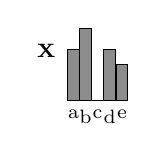
\begin{tikzpicture}
        \begin{axis}[
            ybar,
            axis y line=none,
            axis x line=bottom,
            axis line style={draw=none},
            ymin=0,
            ymax=100,
            width=2.2cm,
            height=2.5cm,
            bar width=1.5mm,
            xtick=data,
            xtick style={draw=none},
            symbolic x coords={a,b,c,d,e},
            xticklabel style={font=\scriptsize, anchor=north},
            axis x line=bottom,
            axis y line=left,
            tick align=inside,
            enlarge x limits=0,
            clip=false,
        ]
            \addplot+[fill=gray!90, draw=black] coordinates {
                (a,70) (b,100) (c,0) (d,70) (e,50)
            };
            \node[
                anchor=south east,
                font=\scriptsize\bfseries,
                xshift=-1mm, yshift=-5mm
            ] at (current axis.north west) {X};
        \end{axis}
    \end{tikzpicture}
}

\newcommand{\bluey}{
    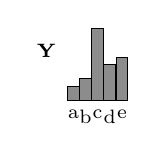
\begin{tikzpicture}
        \begin{axis}[
            ybar,
            axis y line=none,
            axis x line=bottom,
            axis line style={draw=none},
            ymin=0,
            ymax=100,
            width=2.2cm,
            height=2.5cm,
            bar width=1.5mm,
            xtick=data,
            xtick style={draw=none},
            symbolic x coords={a,b,c,d,e},
            xticklabel style={font=\scriptsize, anchor=north},
            axis x line=bottom,
            axis y line=left,
            tick align=inside,
            enlarge x limits=0,
            clip=false,
        ]
            \addplot+[fill=gray!90, draw=black] coordinates {
                (a,20) (b,30) (c,100) (d,50) (e,60)
            };
            \node[
                anchor=south east,
                font=\scriptsize\bfseries,
                xshift=-1mm, yshift=-5mm
            ] at (current axis.north west) {Y};
        \end{axis}
    \end{tikzpicture}
}

\newcommand{\bluez}{
    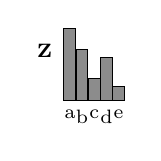
\begin{tikzpicture}
        \begin{axis}[
            ybar,
            axis y line=none,
            axis x line=bottom,
            axis line style={draw=none},
            ymin=0,
            ymax=100,
            width=2.2cm,
            height=2.5cm,
            bar width=1.5mm,
            xtick=data,
            xtick style={draw=none},
            symbolic x coords={a,b,c,d,e},
            xticklabel style={font=\scriptsize, anchor=north},
            axis x line=bottom,
            axis y line=left,
            tick align=inside,
            enlarge x limits=0,
            clip=false,
        ]
            \addplot+[fill=gray!90, draw=black] coordinates {
                (a,100) (b,70) (c,30) (d,60) (e,20)
            };
            \node[
                anchor=south east,
                font=\scriptsize\bfseries,
                xshift=-1mm, yshift=-5mm
            ] at (current axis.north west) {Z};
        \end{axis}
    \end{tikzpicture}
}

\newcommand{\redx}{
    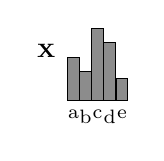
\begin{tikzpicture}
        \begin{axis}[
            ybar,
            axis y line=none,
            axis x line=bottom,
            axis line style={draw=none},
            ymin=0,
            ymax=100,
            width=2.2cm,
            height=2.5cm,
            bar width=1.5mm,
            xtick=data,
            xtick style={draw=none},
            symbolic x coords={a,b,c,d,e},
            xticklabel style={font=\scriptsize, anchor=north},
            axis x line=bottom,
            axis y line=left,
            tick align=inside,
            enlarge x limits=0,
            clip=false,
        ]
            \addplot+[fill=gray!90, draw=black] coordinates {
                (a,60) (b,40) (c,100) (d,80) (e,30)
            };
            \node[
                anchor=south east,
                font=\scriptsize\bfseries,
                xshift=-1mm, yshift=-5mm
            ] at (current axis.north west) {X};
        \end{axis}
    \end{tikzpicture}
}

\newcommand{\redw}{
    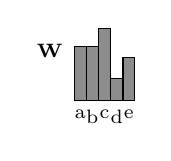
\begin{tikzpicture}
        \begin{axis}[
            ybar,
            axis y line=none,
            axis x line=bottom,
            axis line style={draw=none},
            ymin=0,
            ymax=100,
            width=2.2cm,
            height=2.5cm,
            bar width=1.5mm,
            xtick=data,
            xtick style={draw=none},
            symbolic x coords={a,b,c,d,e},
            xticklabel style={font=\scriptsize, anchor=north},
            axis x line=bottom,
            axis y line=left,
            tick align=inside,
            enlarge x limits=0,
            clip=false,
        ]
            \addplot+[fill=gray!90, draw=black] coordinates {
                (a,75) (b,75) (c,100) (d,30) (e,60)
            };
            \node[
                anchor=south east,
                font=\scriptsize\bfseries,
                xshift=-1mm, yshift=-5mm
            ] at (current axis.north west) {W};
        \end{axis}
    \end{tikzpicture}
}

\newcommand{\redz}{
    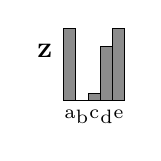
\begin{tikzpicture}
        \begin{axis}[
            ybar,
            axis y line=none,
            axis x line=bottom,
            axis line style={draw=none},
            ymin=0,
            ymax=100,
            width=2.2cm,
            height=2.5cm,
            bar width=1.5mm,
            xtick=data,
            xtick style={draw=none},
            symbolic x coords={a,b,c,d,e},
            xticklabel style={font=\scriptsize, anchor=north},
            axis x line=bottom,
            axis y line=left,
            tick align=inside,
            enlarge x limits=0,
            clip=false,
        ]
            \addplot+[fill=gray!90, draw=black] coordinates {
                (a,100) (b,0) (c,10) (d,75) (e,100)
            };
            \node[
                anchor=south east,
                font=\scriptsize\bfseries,
                xshift=-1mm, yshift=-5mm
            ] at (current axis.north west) {Z};
        \end{axis}
    \end{tikzpicture}
}








\begin{tikzpicture}[node distance=10pt and 20pt, thick]
    % Left side: stacked bar plots with labels
    \matrix (left)[
        matrix of nodes,
        nodes={anchor=west},
        row sep=10pt,
        inner sep=0pt
    ] {
        \node {\bluex}; \\
        \node {\bluey}; \\ 
        \node {\bluez}; \\
    };
    % Draw blue bounding box around left matrix
    \node[draw=blue, thick, inner sep=5pt, fit=(left)] {};
  
    % Middle arrows node, aligned center with left matrix center
    \node[right=1cm of left.center] (middle) {
        \begin{tikzpicture}[thick]
            \draw[->] (-2,3.5) -- (2,3.5) node[pos=0.25, above, yshift=-1mm] {
                \scalebox{0.75}{\bluex}
            };
            \draw[->] (2,2.5) -- (-2,2.5) node[pos=0.25, above, yshift=-1mm] {
                \scalebox{0.75}{\redx}
            };
            \draw[->] (-2,1) -- (2,1) node[pos=0.25, above, yshift=-1mm] {
                \scalebox{0.75}{\bluez}
            };
            \draw[->] (2,0) -- (-2,0) node[pos=0.25, above, yshift=-1mm] {
                \scalebox{0.75}{\redz}
            };
        \end{tikzpicture}
    };
    \node[draw=gray, thick, inner ysep=10pt, fit=(middle)] {};
  
  % Right side: same matrix as left, shifted right of middle
    \matrix (right)[
        matrix of nodes,
        nodes={anchor=west},
        row sep=10pt,
        inner sep=0pt,
        right=2.6cm of middle.center
    ] {
        \node {\redx}; \\
        \node {\redw}; \\
        \node {\redz}; \\
    };
  % Draw red bounding box around left matrix
  \node[draw=red, thick, inner sep=5pt, fit=(right)] {};

\end{tikzpicture}










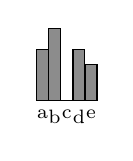
\begin{tikzpicture}
\begin{axis}[
    ybar,
    axis y line=none,
    axis x line=bottom,
    axis line style={draw=none},
    ymin=0,
    ymax=100,
    width=2.2cm,
    height=2.5cm,
    bar width=1.5mm,
    xtick=data,
    xtick style={draw=none},
    symbolic x coords={a, b, c, d, e},
    xticklabel style={font=\scriptsize, anchor=north},
    axis x line=bottom,
    axis y line=left,
    tick align=inside,
    enlarge x limits=0,
    clip=false,
]
\addplot+[fill=gray!90, draw=black] coordinates {
    (a,70) (b,100) (c,0) (d,70) (e,50)
};
\end{axis}
\end{tikzpicture}

\begin{figure}[ht]
    \centering
    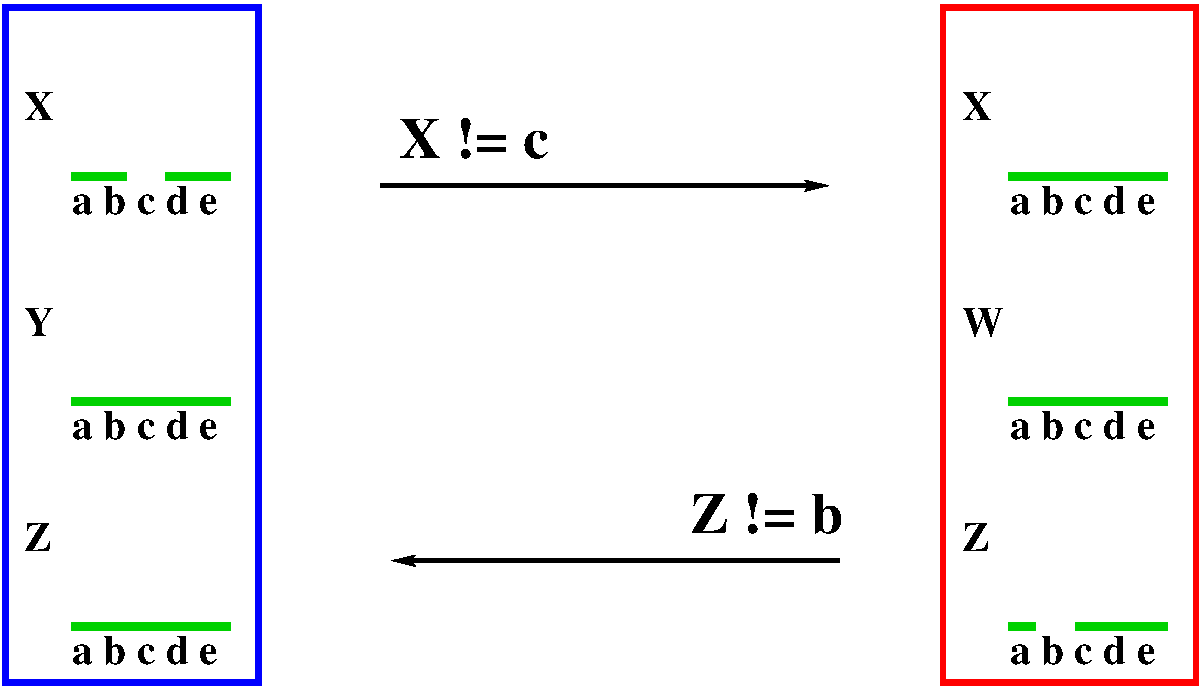
\includegraphics[scale=0.35]{CP-BP-0.pdf}
    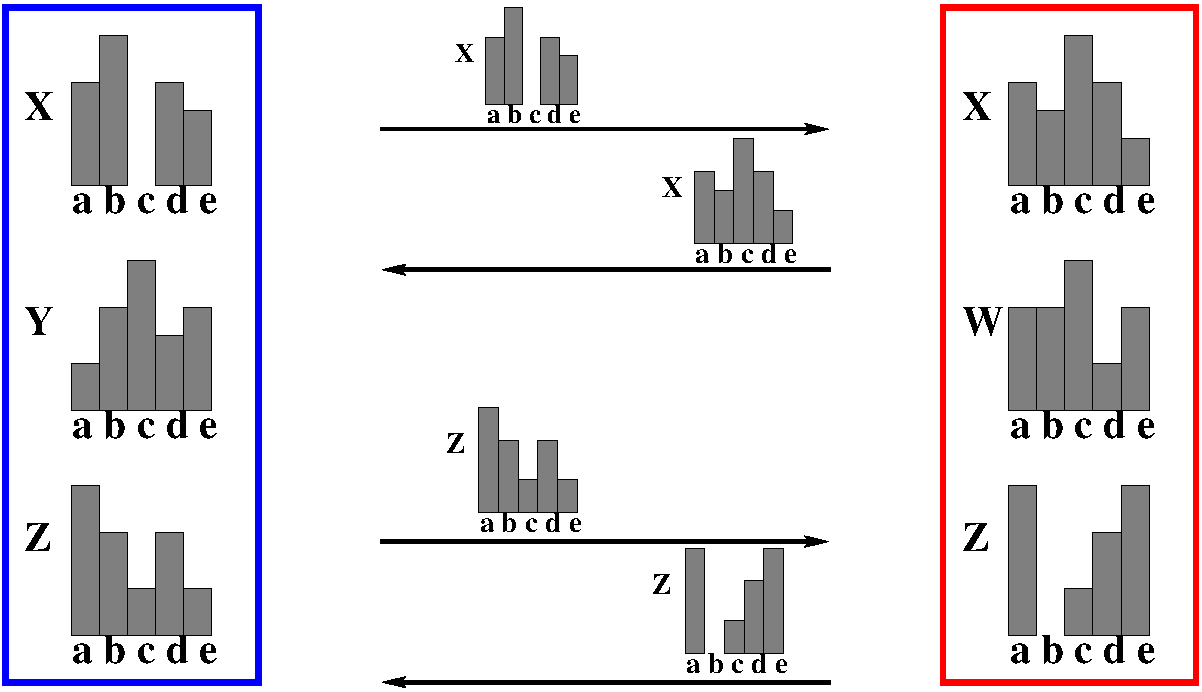
\includegraphics[scale=0.35]{CP-BP-2.pdf}
    \caption[\acrlong{cpbp} messaging.]{Belief Propagation replaces standard constraint messages, which consist of a binary message indicating which values are supported in the domain, with a probabilistic distribution over the domain. As we can see, instead of communicating that the value $c$ for variable $X$ lacks a support, the blue constraint communicates that $X=c$ has a $0\%$ chance of being in a valid solution. This ensures that we can still communicate what values must be filtered out, but we also gain information on the other values in the domain.}
    \label{fig:cpbp_messaging}
\end{figure}


\end{document}